\documentclass[10pt,twocolumn,letterpaper]{article}

\usepackage{cvpr}
\usepackage{times}
\usepackage{epsfig}
\usepackage{graphicx}
\usepackage{amsmath}
\usepackage{amssymb}

% Include other packages here, before hyperref.

% If you comment hyperref and then uncomment it, you should delete
% egpaper.aux before re-running latex.  (Or just hit 'q' on the first latex
% run, let it finish, and you should be clear).
\usepackage[breaklinks=true,bookmarks=false]{hyperref}

\cvprfinalcopy % *** Uncomment this line for the final submission

\def\cvprPaperID{****} % *** Enter the CVPR Paper ID here
\def\httilde{\mbox{\tt\raisebox{-.5ex}{\symbol{126}}}}

% Pages are numbered in submission mode, and unnumbered in camera-ready
%\ifcvprfinal\pagestyle{empty}\fi
\setcounter{page}{1}
\begin{document}

%%%%%%%%% TITLE
\title{Object recognition \& Computer vision \\ Final report - MVA 2015 \\ \textit{Functional Maps: A Flexible Representation of Maps Between Shapes}}

\author{PAUMIER Nicolas\\
ENS Cachan\\
{\tt\small paumiern.ensimag@gmail.com }
% For a paper whose authors are all at the same institution,
% omit the following lines up until the closing ``}''.
% Additional authors and addresses can be added with ``\and'',
% just like the second author.
% To save space, use either the email address or home page, not both
\and
THIS Alexandre\\
ENS Cachan\\
{\tt\small alexandre.this@gmail.com}
}

\maketitle
%\thispagestyle{empty}

%%%%%%%%% ABSTRACT
\begin{abstract} %NICO
%Résumé <= Ce commentaire est utile.
Shape 
\end{abstract}

%%%%%%%%% BODY TEXT

\section{Introduction} %ALEX
%Statement of the problem, quick recap of previous work
One area of interest of shape analysis is the problem of shape matching. The general statement of this problem would be the following : \textit{Given two shapes $S_{1}$ and $S_{2}$, find a mapping that bind the elements of the two shapes}. Once the mapping has been found, there is a wide range of applications that can use it. For example, segmentation transfer can be used in order to find the segmentation of a deformed shape given a segmentation of the initial shape and a mapping between the initial and the deformed shape. Other applications exists such as motion transfer, shape interpolation or statistical modeling for example.\\

The goal of the studied paper is to address the general problem of non rigid shape matching. This problem is quite difficult for several reasons. In contrary to rigid shape matching, the parameters of the transformation are not only tied to rotation and translation anymore. The space of parameters is much higher and it is expensive to optimize the transformation based only on point correspondences. \\

Several paper try to avoid doing this by using different methods that are trying to use only some landmark correspondences in order optimize the transformation, and establish a dense correspondence afterwards. The studied paper is instead focusing on the representation for the correspondences. The goal was to define a compact representation of shape mapping that allows efficient manipulation, that is multiscale and that can lead to simple optimization problems.


\section{Method} %NICO
%Description de la fonctional map
Instead of putting in correspondence points on the shapes, Ovsjanikov \& al propose to consider mapping between functions defined on the shapes. 
Let $T : M \rightarrow N$ be a bijective mapping between manifolds $M$ and $N$. Given a scalar function $f: M \rightarrow \mathbb{R}$, we obtain the corresponding function $g : N \rightarrow \mathbb{R}$ by composition, $g=f \circ T^{-1}$. This induced transformation, $T_F : \mathcal{F}(M,\mathbb{R})\rightarrow \mathcal{F}(N,\mathbb{R})$ where $\mathcal{F}(\dot,\mathbb{R})$ denote a generic space of real-valued function, is the functional representation of the mapping $T$. 

\section{Implementation}
%TODO Recall what has been given, and what has been developped (given : LAB, fast_marching, recomputation of C, knn, ICP)
%Description de comment compute les constraints
\subsection{Laplace Beltrami Operator}
\subsection{Segmention} %NICO
\subsection{Constraints} %ALEX
In order to solve the linear system, one has to compute all the previously stated constraints (function preservation constraints, landmark preservation constraints, segment preservation constraints, and operator commutativity constraints). \\

First, one has to notice that landmark and segment preservation constraints are special cases of function preservation constraints. Indeed, if one wants to add a landmark or a segment preservation constraints, one only need to define functions that are defined on the shapes that are corresponding to point or segment descriptor. In our implementation we used indicator function, distance function to landmarks, and a combination of indicator function and descriptor functions (a function that is $0$ everywhere, and that has the value of the descriptor on the segment for example). \\

We know that the map $C$ bind the functions on the two spaces with the equation $Ca = b$. In order to get a regular linear equation, we rewrote it to have a regular linear equation $Ax = b$ where $x$ is the matrix $C$ written as a vector.\\

The second type of constraints that have been added to the system are the Operator Commutativity constraints. The Laplace-Beltrami operator is being preserved under isometries, therefore we have defined constraints for this operator. Moreover, we rewrote the equation $||L_{2}C - CL_{1}|| = 0$ ($L_{i}$ being the discrete Laplace-Beltrami operator defined on the shape $i$) into a regular linear system $Ax = b$ where $x$ is the matrix $C$ written as a vector. 

\subsection{Weighting of the constraints}
As we have an overly determined system $Ax = b$. Instead of minimizing $e = Ax-b$, we want to minimize $e = W(Ax-b)$ where W is a weight matrix. We can solve the problem by minimizing :
\begin{equation}
e^{T}e = (Ax-b)^{T}W^{T}W(Ax-b)
\end{equation}
This gives a system of linear equations in x :
\begin{equation}
A^{T}W^{T}WAx = A^{T}W^{T}Wb
\end{equation}

Then a linear least square solver has been used to obtain the map C. \\

We finally gravitated toward using the implementation of Pokrass et al. that provide a direct solution to the minimisation problem \textit{minimize $||AX - B||$ s.t. $X'*X = Id$}. Note that the $X'*X = Id$ is the regularization constraints mentioned in our article. Our inspiration for the refinement of the map C is coming from the same open source code. Moreover, in order to find the point-to-point correspondences, we have used an open source kd-tree implementation.
%TODO add reference to licence of flann
%TODO add reference to pokrass, cf licence file



\section{Results} %ALEX
We first decided to test extensively how different constraints could affect the results obtained by this new representation. In order to do this, we used the constraints weighting to selectively choose which functions we wanted to use. Two type of decriptor functions were provided : the heat kernel signature, and the wave kernel signature. For each of those descriptors we had approximately 100 functions. Moreover we did compute different segment in order to add segment constraints. Additionally we tested with some landmark constraints. Moreover we tested the impact of the Operator Commutativity constraints on the results and we also wanted to test how the refinement improved the results. As the refinement does not always converge to the same solution, we computed several refinement of the same map C to analyse the results. Finally we tested quickly the impact of the use of the anisotropic Laplace-Beltrami operator 


\begin{figure}[h]
\centering
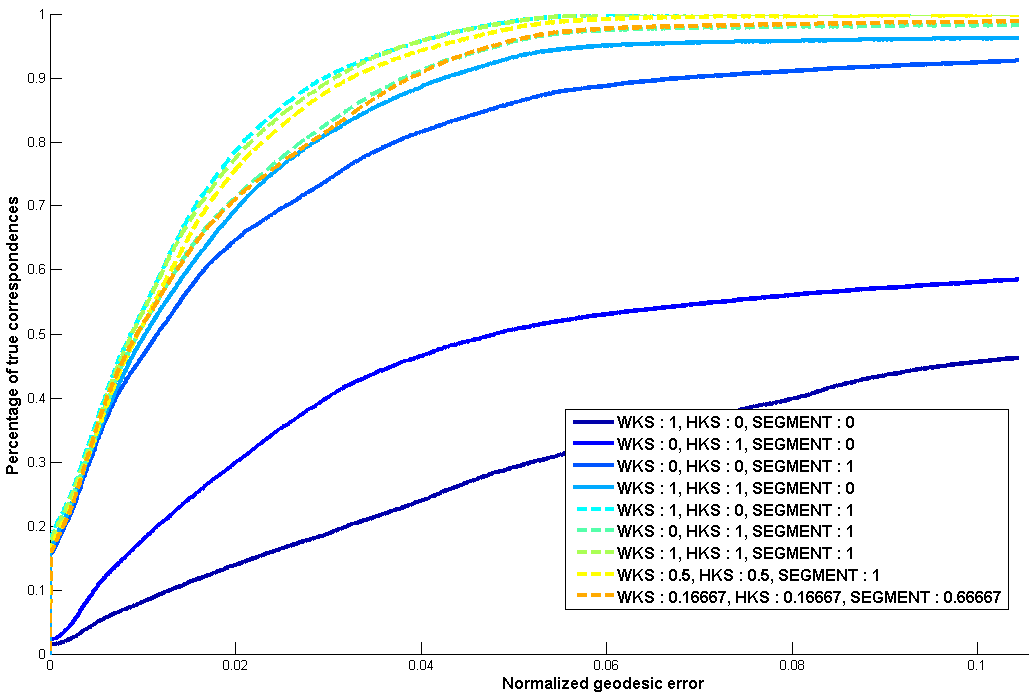
\includegraphics[width=.4\textwidth]{Images/weights.png}
\caption{Impact of the utilisation of the different constraints on the error versus true correspondence}
\end{figure}

%TODO explain



\begin{figure}[h]
\centering
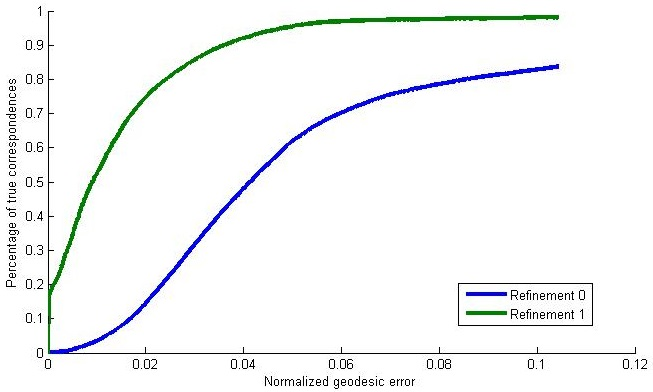
\includegraphics[width=.4\textwidth]{Images/refinement.jpg}
\caption{Impact of the refinement step on the error versus true correspondence}
\end{figure}
%TODO add figure


 

\section{Discussions} %NICO/ALEX
%Analyse des résultats


%-------

{\small
\bibliographystyle{ieee}
\bibliography{egbib}
}

\end{document}
